% This is a template for a Final Year project, which is essentially a 
% document of type "report" with a modified title page
% To create a pdf compile this file using PDFLaTeX. In Texmaker this is 
% the PDFLAT button on the toolbar. You don't need to complie any 
% intermediate formats such as .dvi.
%=========================================================================

%=========================================================================
% This section sets up the standard layout and includes necessary latex 
% packages.
%-------------------------------------------------------------------------
\documentclass[12pt,a4paper]{report}
\usepackage[utf8x]{inputenc}
\usepackage{ucs}
\usepackage{amsmath}
\usepackage{amsfonts}
\usepackage{amssymb}
\usepackage{makeidx}
\usepackage{graphicx}
\usepackage{listings} 
\usepackage[gen]{eurosym}          
\usepackage{url}
\usepackage{fancyvrb}
\usepackage{float}
\floatstyle{boxed} 
\restylefloat{figure}
%\usepackage{minted}
\DefineVerbatimEnvironment{hcode}{Verbatim}{fontsize=\small}
\DefineVerbatimEnvironment{hexample}{Verbatim}{fontsize=\small}
\newcommand{\ignore}[1]{}


\begin{document}

%=========================================================================
% In
%-------------------------------------------------------------------------
%=========================================================================
% This contains basic project information (Title/Author/Supervisor etc.)
% which should be filled in by the student.
%-------------------------------------------------------------------------
\newcommand{\inProjectTitle}{Implmenting a interpreter for a scripting lanaguge using Haskell}
\newcommand{\inInterimReport}{Final Year Project Report}
\newcommand{\inAuthorFName}{Zhen}
\newcommand{\inAuthorLName}{Lao}
\newcommand{\inAuthorEmail}{zhen.lao@student.dit.ie}
\newcommand{\inSupervisorFName}{Richard}
\newcommand{\inSupervisorLName}{Lawlor}
\newcommand{\inSecondReaderFName}{Cindy}
\newcommand{\inSecondReaderLName}{Liu}			% student edits this - title, name, email etc.
%=========================================================================
% This lays out the title page. 
% DO NOT EDIT THIS PAGE except to uncomment the text below -  
% "This Report is submitted..." to reflect the programme title.
%-------------------------------------------------------------------------

% Commands to make entry and formatting of Title/Author info more intuitive
\newcommand\ProjectTitle[1]{\begin{LARGE}\textsc{#1}\end{LARGE}\\[1.25cm]}
\newcommand\InterimReport[1]{\begin{LARGE}\textsc{#1}\end{LARGE}\\[1.25cm]}
\newcommand\AuthorName[2]
{\begin{LARGE}#1 \textsc{#2}\end{LARGE}\\[0.25cm]}
\newcommand\AuthorEmail[1]{\begin{Large}\texttt{#1}\end{Large}\\[0.75cm]}
\newcommand\Supervisor[2]{\begin{large}\textit{Supervisor: }#1 \textsc{#2}\end{large}\\[0.25cm]}
\newcommand\SecondReader[2]{\begin{large}\textit{2nd Reader: }#1 \textsc{#2}\end{large}}

\begin{titlepage}
\begin{center}

% Upper part of the page contains DIT logo disable the dit logo

\includegraphics[scale=0.60]{pic/s1.png}\\[2.5cm]
 
% Title 
\ProjectTitle{\inProjectTitle}
\InterimReport{\inInterimReport}
% Author and supervisor
\AuthorName{\inAuthorFName}{\inAuthorLName} 
\AuthorEmail{\inAuthorEmail}
\Supervisor{\inSupervisorFName}{\inSupervisorLName}
\SecondReader{\inSecondReaderFName}{\inSecondReaderLName}

% Bottom of the page
\vfill
{\large \today}\\[0.5cm]  % Date compiled

This Report is submitted in partial fulfillment of the requirements for the award of the degree of
\textbf{BSc Computer Science}  % DT228
% \textbf{BSc Computing}  % DT211
of the School of Computing, College of Sciences and Health, Dublin Institute of Technology.
\end{center}
\end{titlepage}			% no editing required here

% Abstract 
\begin{abstract}
Haskell is purely functional programming language.Programmer can build larger programm from small modular and building block.In thesis,we will talk about the process and technologies to build a scripting programming language called \textbf{yun} using Haskell.Monad and monadic transformer are to fundamental concept for us to build the programming we will be discuss in chapter 4-5.
\begin{flushleft}
\textbf{Keywords:}programming language,monad,monad transformer,functional programming,\textbf{yun}
\end{flushleft}
\end{abstract} 
%=========================================================================
% This contains a declaration that the student has complied with the rules  
% regarding plagairism. The paper copy of this page must be signed by the 
% student and supervisor before submission.
%-------------------------------------------------------------------------
\section*{Declaration}
I \textbf{\inAuthorFName} \textbf{\inAuthorLName} hereby declare that the work described in this dissertation is, except where otherwise stated, entirely my own work and has not been submitted as an exercise for a degree
at this or any other university.


\vfill

\begin{tabular}{ l p{4cm} }
Signed &  \\ \cline{2-2}
 & \textit{\inAuthorFName}  \textit{\inAuthorLName} \\ [2.0cm]
\end{tabular}

\pagebreak		% needed because next (probably Acknowledgements) is a section not a chapter			% needed only if the document must have a Declaration
% Acknowledgements
\section*{Acknowledgements}
I would like to thank my supervisor Richard Lawor,for his valuable advice and useful suggestions on my project.\\
I am also deeply indebted to all the other tutors and teachers in Computer Science for their direct and indirect help to me.\\
Special thanks should go to my friends who have put considerable time and effort into their comments on the draft. 

%=========================================================================
% Use the next 3 commands to include Abstratct/Declaration/Acknowlegdements in 
% the table of contents 
%-------------------------------------------------------------------------
%\addcontentsline{toc}{section}{Abstract}
%\addcontentsline{toc}{section}{Declaration}
%\addcontentsline{toc}{section}{Acknowledgements}

%=========================================================================
% Autogenerate tables of contents, figures and tables
%-------------------------------------------------------------------------
\tableofcontents
\listoffigures
%\listoftables
%\lstlistoflistings

%=========================================================================
%  Set up environment for code listings
%-------------------------------------------------------------------------
\lstset{
	basicstyle=\small,          			% print whole listing small
	keywordstyle=\bfseries\underbar,		% bold underline keywords
	stringstyle=\ttfamily,      			% typewriter type for strings
	identifierstyle=\bfseries,				% bold identifiers
	showstringspaces=false,     			% no special string spaces
 	numbers=left, 
	numberstyle=\tiny, 
	stepnumber=1, numbersep=5pt,
	breaklines,
	breakatwhitespace	
	}

%=========================================================================
% Actual chapters start here.
% 
% The basic idea is that each chapter is a separate .tex file which is 
% included at compile time. Each file should have a meaningful filename.
%-------------------------------------------------------------------------
\chapter{Introduction}
\section{Objective and Motivation}
The objective of this project is to develop a weak-type interpreted language using Haskell.This language is able to support the following feature,
\begin{itemize}
\item basic for loop and while loop
\item basic if-else statement
\item functional invocation 
\item arbitrary dimension list
\item polymorphic list
\end{itemize}

Furthermore, in project,the monadic design approach is applied as Haskell is different from other object oriented language.

\section{Benefits of using Haskell} 
Haskell is an advanced purely-functional programming language.By applying the used of Haskell to this project ,I have significantly reduce the coding time and spent most of my time to the design phrase.
\subsection{Function As First Class Member}
A pure function is a function that accept an input and generate  an output.In Object-Oriented language,program are constructed using class and instance which encapsulate computation and state.Haskell program is construct by function as function is the first class member in Haskell.Typically the main function is defined in terms of
other functions, which in turn are defined in terms of still more functions, until at the bottom level the functions are language primitives. All of these functions are much like ordinary mathematical functions.
[Why Functional Programming Matters]

\subsection{Monad}
However,Haskell has to deal with in-pure operation like state and IO.

\section{Development Methodology}
Agile development methodology is used in the entire development process.This project has been initially identified multiple iteration and each iteration contains three major stages research ,development and testing.
\chapter{Technologies}
\section{Parsing technologies}
\subsection{Formal Grammar}

Mathematically, formal grammar consists of:
\begin{itemize}
\item a finite set of terminal symbols.
\item a finite set of non-terminal symbols.
\item a finite set of project rules.
\item a start symbol.
\end{itemize} \cite{aho1986compilers}
[Three Models for the Description of Language]
From the formal grammar definition, legitimate production rules can be written as 
 \[ S \mapsto aS  \,and \, S \mapsto ab \]
In this example,we can assume that the grammar consists of two projection rules and the starting symbol is $ S $.The terminal symbols are lower letters $ \{a ,b\} $ . From this example, If we start from the either rule 1 or rule 2 ,we could derive a  grammar of $ \{ a^n b | n>1  \}$ ,which can be enumerate like $ \{aab,aaab,aaaab,\cdots \} $.



%In addition,we are able to write all the production rule from the given abstract %language, the language like

\subsection{Context-Free Grammar}
Context-Free Grammar (CFG)
A context-free grammar is has four component
1. A set of terminal symbols, sometimes referred to as ”tokens.” The
terminals are the elementary symbols of the language defined by the
grammar .
2. A set of non-terminals, sometimes called ”syntactic variables.” Each
non- terminal represents a set of strings of terminals, in a manner we
shall describe.
3. A set of productions, which are rules for replacing (or rewriting) non-
terminal symbols (on the left side of the production) in a string with
other non-terminal or terminal symbols (on the right side of the pro-
duction).
4. A start symbol, which is a special non-terminal symbol that appears
in the initial string generated by the grammar.
[?] Context-free grammar can be recognized by pushdown automaton.




\subsection{The Hierarchy of Grammars}
Noam Chomsky has describe three model of grammar ["Three models for the description of language"]  and this grammar model has significantly effect the design of computer programming language.


Chomsky define a set of rule upon the formal grammar and categorize them into different levels.

The Chomsky hierarchy consists of the 4 levels:
\begin{itemize}
\item Type-0 grammars (unrestricted grammar). It is a unrestricted grammars that include all possible grammar that are possible to recognize by Turning machine.
\item Type-1 grammars (context-sensitive grammar).if all rules are of the form $  \alpha A \beta \rightarrow \alpha \gamma \beta$ where $ \alpha \,  \beta \, \gamma $ are terminal symbols and $ A $ is non-terminal symbol.
\item Type-2 grammars (context-free grammar). 
\item Type-3 grammars (regular grammar).
\end{itemize}

\subsection {Backus–Naur Form and Extended Backus–Naur Form}
The Backus-Naur Form(BNF) is a metalanguage to write the production rule that expressing the type-2 grammar (context-free grammar).It  restricts the appearance of terminal and non-terminal in each side of the production equation.A canonical BNF production rule may like follow,
 \[   <symbol> ::= \_\_expression\_\_ \]
 
The left side of the equation can only be non-terminal thus enclosed with $<>$ .The right hand side can be terminals and non-terminals,a vertical bar '|' is used to represent choice between terminal and non-terminals.\\

The  Extended Backus–Naur Form (EBNF) and extension upon the BNF.Three regular expression qualifier is added to simplified some expression,they are,
\begin{itemize}
\item ? : which means that the symbol (or group of symbols in parenthesis) to the left of the operator is
optional (it can appear zero or one times)
\item * : which means that something can be repeated any number of times (and possibly be skipped
altogether)
\item + : which means that something can appear one or more times 
\end{itemize} \cite{book}

Recrusive rules of BNF  like 
\[   1. <exp> := <exp> | sub \]
\[	 2. <exp> := sub     \]
 
that expressing a sequence of a particular syntactic element can be simplified using quantifier in EBNF as $ <exp>:=sub+ $



\section{Parser Generator Haskell Happy}
Happy is a parser generator system for Haskell, similar to the tool `yacc' for C. Like `yacc', it takes a file containing an annotated BNF specification of a grammar and produces a Haskell module containing a parser for the grammar.
[The Parser Generator for Haskell] 

By using its own EBNF like syntax,used could write an parser description.The happy parser generator are able to recognize and compile it into Haskell source code.


\section{Monadic Parsing using Parsec}
In the early stage of this project,parse is build using parse C,
Parsec is an industrial strength, monadic parser combinator library for Haskell. It can parse context-sensitive, infinite look-ahead grammars but it performs best on
predictive (LL[ Compilers: principles, techniques and tools.]) grammars. Combinator parsing is well known in the literature
and offers several advantages to YACC or event-based parsing. [Parsec, a fast combinator parser] 

Compared toe parser generator , monadic parsing has two major benifits
1. No need to learn additional parser generator grammar since parser combinator is written in the same language. 2.parser can be adjust easily .




\section {Lexical analysis}
Before parsing,the lexical analyser will scan the source code and generate a sequence of tokens.The tokens are often defined by regular expressions.

For example,the statement \textbf{s3 = s1 + "a string"} will be parse to tokens,

\begin{tabular}{|c|c|}
\hline s3 & identifier ,variable name \\ 
\hline = & operator \\ 
\hline s1 & identifier,variable name \\ 
\hline + & opeartor \\ 
\hline "a string" & a string constant \\ 
\hline 
\end{tabular} 


The regular expression $ [a-zA-Z]{1}[a-zA-Z\setminus\_0-9]*  $ can identify strings that begin will alphabetical character.


\subsection{The Lexer Generator Alex}
Alex is a tool for generating lexical analysers in Haskell, given a description of the tokens to be recognised in the form of regular expressions. It is similar to the tools lex and flex for C/C++.
\\\\
Alex takes a description of tokens based on regular expressions and generates a Haskell module containing code for scanning text efficiently. Alex is designed to be familiar to exisiting lex users, although it does depart from lex in a number of ways.
[Alex User Guide  ]

\section{Testing and Evaluation Technologies}
There are two type of testing in Haskell.The type testing and unit testing.There correspond to two package in Haskell,QuickCheck and HUnit.
\subsection*{QucikCheck}
For pure functions programmer can write logical expression or functional specification to prove the code is correct ranter than provide a specify test case as an input of the function.
One of the example to test a function that takes the first five element of a list is using a length function $ if \;\forall \;s.\; length(take5 \;s) = 5 \;$ is true,then the $take5$ function is probably true.
The QuickCheck package allow us to write the assertion in Haskell code this way.
\begin{hcode}
quickCheck (\s -> length (take5 s) == 5)
\end{hcode}

\subsection*{HUnit}
HUnit is a unit testing framework for Haskell to test the impure code.it is similar to the JUnit tool for Java.In unit testing,it is required to provide an input and verify the output.



\chapter{Monad in Haskell}
\section{Haskell and Category Theory}
Category theory is a general theory that examine and organize mathematical object like set ,function,function domains Cartesian-set.

A Category $C $ in category theory is defined below :
\begin{enumerate}
\item a collection of objects 
\item a collection of arrows (often call morphism) 
\item operations assigning to each arrow $f$ an object $dom\;f$,its domain ,and an object $cod\;f$,its co domain.
\item a composition operator assigning to each pair of arrows $f and g$,with $cod\;f = dom\;g$,a composite arrow $ g \circ f:dom\;f \rightarrow  cod\;g$ , satisfying the following associative law: \\
For any arrow $f: A \rightarrow B,g:B \rightarrow C,and\;h: C\rightarrow D$(with A,B,C and D not necessarily distinct),
$$h\circ (g\circ f) = (h\circ g)\circ f$$
\item for each object A, an identify arrow $id_{a}: A \rightarrow A$ satisfying the following identity law:\\
For any arrow $ f: A \rightarrow B,$ 
$$ id_{a} \circ f = f  \;and\;  f\circ id_{a} = f. $$
\end{enumerate}\cite{pierce_basic_1991}

Functions are the first member of the program in functional programming,since no size affect is not allow ,there should be a way to combine the all kinds of functions to from a new function instead of just simply chain the input output of each function as the former will generate intermediate output.


For instance ,counting the file of java source code in current directory can be written as follow:


	$$ ls-al . | grep *.txt| wc -l $$ 
	
	
To substantiate the this concept , let's use the map/fold fusion technique of Haskell as an example.

If we want to calculate the sum of the square of each element of a list eg. [1,3,4,6,7,9],the result of it is  $ 1^2+3^2+4^2+6^2+7^2+9^2=192 $.In Haskell ,we could use map and fold to address problem.

 %list_of_square = map (^2)
%sum_of_list = foldr (+) 0
%sum_of_square =   sum_of_list.list_of_square

To avoid generating intermediate output from the first function to second function, the could rewite the hold function using a single fold

The all map/fusion is is equivalent to 
$ foldr f e . map g = foldr (\\x y -> f (g x) y) e $

therefore, the 

$ sum_of_square = foldr (\\x y -> x^2 + y) 0 $





\section{Monadic Function}
\section{Using Monad Operator to Combine Monadic Function}

\section{Type system in Haskell}
\section{Do Notation - Reinventing a imperatilanguageve language}


\chapter{Monad Transformers}
\section{Overview}

As we already have monad designed to model side-effect with restricted type,it would not be too much problem to perform an action using monad in Haskell.New monad might be needed form operation that are able to perform state manipulation as well as IO action.\\

Monad transformers offer an additional benefit to monadic programming: by providing a
library of different monads and types and functions for combining these monads, it is possible
to create custom monads simply by composing the necessary monad transformers. [Monad Transformers Step by Step]\\

In real world application, it is often the case that a combination different type of action is required to put into one function.Monad transformer provide a new way to glue them together.

\section{State Transformer}
A value of type \textbf{(ST a s)} is a computation which transforms a state index by type s ,and delivers a value of type a ,You can think of it as a box ,like this 
\begin{figure}[H]
  \centering
	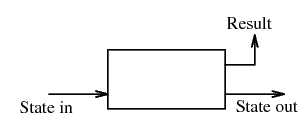
\includegraphics[width=0.60\textwidth]{pic/c3/state.png}
	\caption{Diagram illustrating a state monad}
\end{figure}
[lazy functional state thread]
\\

First , a state transformer is a monad, other than encapsulating a data behind signature , it encapsulated a computation,the \textbf{runState} function provide by the state monad is an escape function that allow us to extract is state logic from the computation,by feeding the state computation function with an initial state,we are able to get the final state.Other type of escape function is provided to extract computation as well.

Second,a state transformer can accept other monads to combine the computation which state as well as other logic says the IO logic.


\section{Error Transformer}
ErrorT monad transformer can be used to add error handling to another monad.
The ErrorT monad type constructor is ,
\begin{hcode}
newtype ErrorT e m a
\end{hcode}
The first parameter e is the error type like the Either Monad constructor ,m is the inner monad,a is the type of the computation.

\begin{hcode}
instance (Monad m, Error e) => Monad (ErrorT e m) where
    return a = ErrorT $ return (Right a)
    m >>= k  = ErrorT $ do
        a <- runErrorT m
        case a of
            Left  l -> return (Left l)
            Right r -> runErrorT (k r)
\end{hcode}

From the definition above , we can derive its bind strategy which is the most important thing for us to understand a monad.For two computation \textbf{m} and {k},the bind strategy is  that it will try to extract the result from the first computation which might return a error message ,the whole computation will fail on the first computation which will attempt on the succeed of the first.computation.

The escape function \textbf{runErrorT} can help us to extract the inner level monad which is a computation with some kinds of monad logic and execute it.

\section{Combining Monads}
Monad transformers create a new monad by extending an existing monad with additional operations, thereby allowing new programming language features to be de defined while preserving any language definition given for the original monad.[Modular Compilers Based on Monad Transformers]\\ 

As monad guarantees the correctness of the computation with the type restriction,namely we can not combine two computations one with "stateful" while other with IO logic into one building block,we might need addition functions like lift and liftIO together with monad transformer to fix the type problem .\\


As we can imagine that, if could combine every monad for most of monad if offer a monad transformer form.In this way,the action combine inside to notation would probably be no different from a real imperative language.When we combine all monads, the type restricted become slacked accepting a type of computation with side effect which is no difference from a real imperative language.\\

The only difference might be the sequence we encapsulate monad and monad transformers,that is we can only warp IO inside other monad transformers.

\chapter{Language Interpreter Design}


\section{Imperative and Declarative language}




\section{Type System}
\subsection{Dynamic Typing and Static Typing}
A programming language is said to use static typing when type checking is performed during compile-time as opposed to run-time. 
For example , you have to specify the type explicitly and the compile will the the type correctness of a variable.A variable of a specified type can not assign to another value of other type.

\begin{tabular}{p{5cm}|p{5cm}}
\hline
Static Typing & Dynamic Typing \\
\hline
int a =1;\par \textbf{/*a is of type int */} \par int a="a string"; \par \textbf{ /* its not valid to assign a string to a variable that has type int */} & a=1; \par \textbf{/* does not need to specified a type for this variable */} \par a ="a string"; \par
\textbf{/* it valid to change the type of the variable */} \\ 
\hline
\end{tabular} \\\\
In my project, I used the dynamic typing scheme,which is ,does not need to specify any type of variable and able to assign any type of primitives to a variable.

\subsection{Strong Typing and Weak Typing}
a language is said to be strong typing is that it place restriction in operation where data type can not be intermix.


\begin{tabular}{p{6cm}|p{6cm}}
\hline Strong Typing & Weak Typing  \\ 
\hline a=123; \par 
\textbf{/* a is a number */} \par 
b="123" \par  
\textbf{/* b is a string */} \par 
c=a+b \textbf{/* return type error */}  &  
a = 123; \par 
b = "123"; \par
c = a+b; \par 
\textbf{/* either a will be convert to a string or b will be convert to a number */}

\\ 
\hline 
\end{tabular} 

In my project,I have implemented a weak typing system .I have design an statement call generic expression , which allow different kinds of value to intermix with each other. An expression like "12343" + 1232 -324 can be parse as follow syntax tree.





\section{Problem and resolution in writing BNF/EBNF rules}
\subsubsection{Shift//Reduce Problem}

\subsubsection{Reduce//Reduce Problem}



\chapter{Language Implementation}


\section{Data Type}
\subsection{Tokenizer Type}
All tokens are define using the Haskell Lexer Generator Alex.Tokens will be recognized and converted to Haskell data types.For example , a valid variable is comprised with one or more alphabetic characters and digit and the first character must be an alphabetic characters. This rule can be defined as ,
\begin{lstlisting}[language=java]
$digit = 0-9			-- digits
$lowerCase = [a-z]
$alpha = [a-zA-Z]		-- alphabetic characters

tokens :-
  $alpha [$alpha $digit \_ \' \.]* { \s -> TName s }
-- data definition
data Token = 
	TName String |
	TBool Bool  | 
	TInt Int  | 
	...  -- more definition			

\end{lstlisting}

The variable \textbf{var1} will be parse into Haskell data type \textbf{TName "var1"}\\


By using the lexer , all the code will be generated into tokens streams.
\begin{lstlisting}[language=java]
program myProgram ()
{
	var1 = 1;
	result = var1 + "a string";
}
\end{lstlisting}

The following codes show the invocation of the lexer and the returned tokens stream.
\begin{lstlisting}[language=java]
lexer "program myProgram() { var1 = 1; result = var1 + False; return 0; }"
[TProgram,TName "myProgram",TOPB,TCPB,TOCB,TName "var1",TAssign,TInt 1,TSC,TName "result",TAssign,TName "var1",TPlus,TBool False,TSC,TReturn,TInt 0,TSC,TCCB]
\end{lstlisting}



\subsection{Parser internal data type}
The Parser internal data type typically represents a parse tree.To represent a generic expression,we can define data type as follow,

\begin{hcode}
data GenericExp  =
		     Var String 
		   | Int Int
		   | Double Double
		   | Plus GenericExp GenericExp		   
		   | ListIndex String [GenericExp]
		   | Brack GenericExp  deriving 
		   ... -- more definition
\end{hcode}


The following code 
\begin{lstlisting}[language=java]
( a +1 )  /=  3
myArray[ 1+1,2] 
\end{lstlisting}

are parsed into Haskell data structure,

\begin{hcode}
NotEq  (Brack ( Plus (Var "a") (Int 1)))  (Int 3)
ListIndex "myIndex" [ Plus (Int 1) (Int 1) , Int 2 ] 
\end{hcode}


\begin{figure}[H]
  \centering
	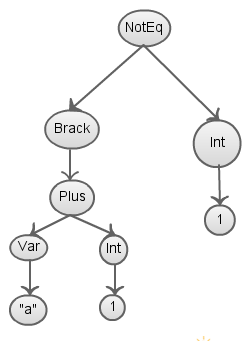
\includegraphics[width=0.40\textwidth]{pic/c6/parse_tree_1.png}
	\caption{Diagram illustrating a parse tree of a generic expression}
\end{figure}


In Haskell,a parse tree data structure that support polymorphic list can be defined using recursive data type as follow, 
\begin{hcode}
data List = ListGenericExp GenericExp
			| ListList [List] deriving (Show,Eq,Read)  
\end{hcode}


A polymorphic list,
\begin{lstlisting}[language=java]
 [1,2,["string",2,3]];
\end{lstlisting}

Can be represent in Haskell data type.

\begin{hcode}
ListList  [ListGenericExp (Int 1),ListGenericExp (Int 2),
	ListList [ListGenericExp String "string",
		ListGenericExp (Int 2),ListGenericExp (Int 3)]] 
\end{hcode}



\begin{figure}[H]
  \centering
	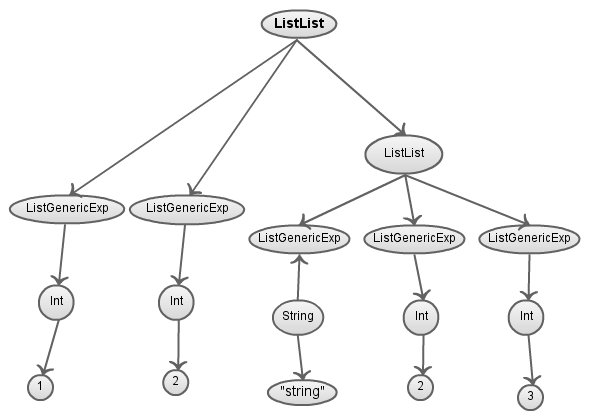
\includegraphics[width=0.90\textwidth]{pic/c6/parse_tree_2.png}
	\caption{Diagram illustrating a parse tree of a list expression}
\end{figure}


\subsection{Interpreter Internal Data Type}
The data type defined as below shows that the possible data type of result that a sub-interpreter will return.There is a interpreter correspond it.The sub-interpreter will return for example an interger to represent the result of a generic expression.The recursive data type is use for a the purpose of nested list support. 
\begin{hcode}
data Value =  Int Int 
             | Bool Bool
             | Double Double
             | String String 
             | List [Value]
             | NULL    deriving Show
\end{hcode}


\subsubsection{The Interpreter Monad}
The interpreter monad is a combination of Error Monad ,State Monad and IO monad.

\begin{hcode}
type Interp a  = (ErrorT String (StateT Storage IO )) a

type SymbolTable = M.Map String Value
type Storage = (SymbolTable,[Func])
\end{hcode}


For each sub-interpreter ,it must accept an expression and return a \textbf{Interp} type.The \textbf{Interp} type is a monad constructor that offer encapsulation support to return value.One of the \textbf{StateT} parameter is the type \textbf{Storage} which represents the internal storage of an interpreter like symbol table and parse tree of sub-function.



\section{Module Evaluator}
Module is the minimum executable unit in \textbf{yun} programming language.A module is comprised by one main function and multiple sub functions.What the Module Evaluator will do is ,first initial the symbol table using a empty map, second, extract the parse tree data and put in two together with the symbol table,third,extract all statements in main function and hand it over to statement evaluator.This Evaluator will not check the error message from other sub-evaluator it invoked,all the error will be passed to the main function.
\begin{figure}[H]
  \centering
	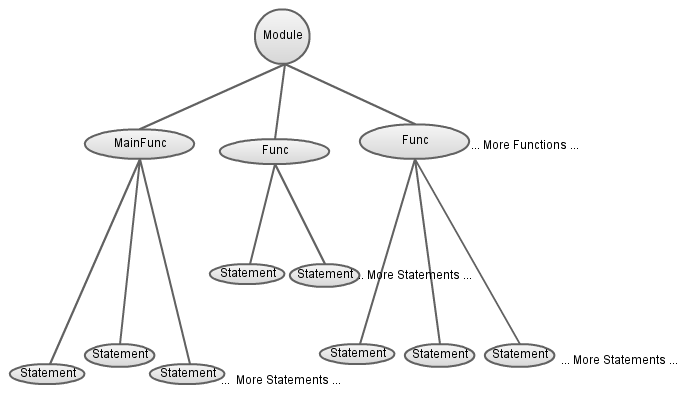
\includegraphics[width=0.90\textwidth]{pic/c6/module.png}
	\caption{Diagram illustrating a parse tree of a module}
\end{figure}
\section{Statement Evaluator}


\begin{hcode}
data Control = Break | Continue | DoNothing | Return Value deriving (Show)

stmtsEval :: [Stmt] -> Interp Control
stmtsEval --   function body

stmtEval :: Stmt -> Interp Control
stmtEval  -- the function body
\end{hcode}
\textbf{Stmt} is a data type that represents a Parse Tree of a statement.The first statement evaluator will accept a list of statement and for each statement,it invoke the statement evaluator.By applying patter matching,the statement will do correspond action toward each type of the statement.For example, for the \textbf{break} or \textbf{continue} statements,it will return the corresponding control command.The diagram below illustrate the how the statement evaluator works.

\begin{figure}[H]
  \centering
	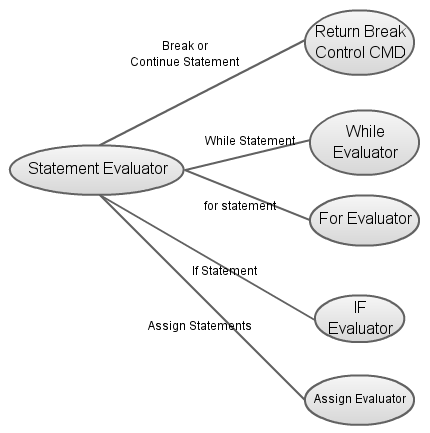
\includegraphics[width=0.80\textwidth]{pic/c6/statement.png}
	\caption{Diagram illustrating guard condition and function invocation}
\end{figure}




\section{Symbol Table and Parse Tree}
The symbol table together with the parse trees of sub-functions as a tuple will be stored behind the state monad.Symbol table is a map that mapping from a string to the type \textbf{Value} mentioned above.


\section{Generic Expression Interpreter}

\subsection{Function Invocation}
\section{Main Function}
\chapter{Analysis,Conclusion and Future Work }
\section{Analysis}
In the initial stage of this project,lots of possibility has been considered ,for instance,the parsec parser library and happy parser generator library.What's more, I also need to design which this programming language need to be a static type of dynamic type language.As there is lots of debate in pros and cons on various type system, I make the choice simple base on the difficult of implementation of a certain manifold.\\

The puerility and monad also help me a lot in writing this project.In this project,on a small amount of function is pure and most of other are monadic function as in this project,I made use of the monadic design approach.The monadic design approach helps me to limit to side-effect into monad and I can specify to limit the type of side-effect.
\\

Above all,Haskell is a suitable language to do this project which is a important reason for the success of this project.



\section{Conclusion}
Haskell is a high-level language and provide a lots of tools to glue functions together thus can implements functionality elegantly.\\

Haskell's type system has placed numerous restrictions on my code and it turn out to be when I try to implements something new in project , most of time, when I passed the compiling phrase I can have correct implementation.\\

In the passed three years, I have learnt quit few of programming language.By doing this project,I can be on a on the side of language design rather than a user, to review other languages' features and characteristic I have leant.It allows me that think about how a language is implemented and why it was implemented this way.\\

There are great amount of disputes on pros and cons between different programming languages.Those disputes, to a large extend, have ignored the fact that programming languages are created for computer scientist to resolve problem.


Compared to imperative programming paradigm,its obvious that the functional programming paradigm is not von Neumann related.For a von Neumann style programming, to construct a program,we have to write command to continuously modify the state of a memory cell to achieve ,for instance ,changing a pixel's color on the screen.Functional programs deal with structured
data, are often nonrepetitive and nonrecursive, are hierarchically constructed,do not name their arguments, and do not require the complex machinery of procedure declarations to become generally applicable. Combining
forms can use high level programs to build still higher level ones in a style not possible in conventional languages.\cite{liberate}


\section{Future Work}
This project can be extended to a Domain-specific language (DSL) which is a language designed delicately to particular program domain.Logo a dialect of Lisp and was created for education purpose.This language allow programming to draw shapes on the screen.To build a DSL,a research needed to be conduct for a specified domain ,additional syntax and primitives needed to be added into the language.For example,Haskore is a clean and elegant notation for music information and structure.In this framework, musical objects consist of primitive notions such as notes and rests, operations to transform musical objects such as transpose and tempo-scaling, and operations to combine musical objects to form more complex ones, such as concurrent and sequential composition. \cite{music}
 \\\\
With Haskell powerful support abstraction support like monad , high-order function and function composition, implementing a language is not so painful.
Though the current project is only focus on a generic purpose language , other people has implemented lots of  Domain-specific language hosted by Haskell runtime,for instance ,KURE is a Haskell hosted Domain-specific Language (DSL) for writing transformation systems based on rewrite strategies.\cite{hosted}\\\\
A DSL is created for resolving problem that is easy to design and tedious to implements and Haskell is the best candidate to do this job.\\

Therefore, I would like to put this topic in  future work part.As form Haskell,creating new grammar with the powerful tool it already provided is straight forward and convenient.
 
%\chapter{Future Work and Project Plan}
\section{Future Work}
I have done most of the research work of the project.the future work will be implementing the actual parser.There will be an initial implementation of part of the EBNF definition.The execution engine will be implemented at the same as the parser.Due to Haskell have a powerful abstraction mechanism and a suitable library (Parsec),the implementation will not be too difficult.

The major barrier will be implementing the execution engine since I have no knowledge about it.
There will be more research in the later stage of this project on the interpreter part as well as the grammar and Haskell part.

\section{Project Plan}
\begin{tabular}{|p{1.00\textwidth}|}

\hline \textbf{Before November} \\
I have finish most of research on Chomsky's 
CFG grammar and Haskell.I have started to implement a prototype of the interpreter.\\

\hline \textbf{November 12 to November 26}\\
Research on the execution engine of the interpreter.\\
\hline \textbf{November 12 to November 31} \\
Development a prototype by following the documentation of parsec. The document  "Write Yourself a Scheme in 48 Hours/Parsing" offer an example to implements a interpreter for Scheme using parsec library of Haskell.\\
\hline
\textbf{November 31 to January 15} \\
Implement a subset of EBNF specification of $yun$.Add the error checking to the interpreter.Meantime,as the code growing ,unit test will be added to guarantee the quality of existing code.
\\
\hline  \textbf{January 16 to February 15}\\
Implement all the EBNF specification of $yun$\\
\hline   \textbf{February 31 to March 15}\\
Implement the IO command (library).Add more test code.\\
\hline \textbf{February 16 to March 16}\\
Review the EBNF of $yun$ programming language.Implement more library for it.Start the system testing.
\\ 
\hline \textbf{March 17 to April 8}\\
Prepare for the project fair.\\
\hline
\end{tabular} 









%=========================================================================
% This section renders the bibliography
%-------------------------------------------------------------------------
\clearpage										% these two lines needed to add Bibliography
\addcontentsline{toc}{chapter}{Bibliography}   	% to Table of Contents
\bibliographystyle{plain}
\bibliography{Biblio1} 		% You can include multiple files. 
							% There is no whitespace between the commas and the next bib file.


%=========================================================================
% Everything after here is an appendix
%-------------------------------------------------------------------------
\appendix	

%\input{References.tex}
%\input{Glossary.tex}
%\chapter{Appendix}
\section{Environment setup}
\begin{lstlisting}[language=bash]
sudo apt-get install haskell-platform
# install haskell-platform
sudo cabal install happy
sudo cabal install alex

cd PATH_TO_PROJECT
#change path to project directory

happy -i grammar/Grammar.y
alex grammar/Lexer.x
ghc --make -i"test" -i"src" -i"grammar" "src/Main.hs" -outputdir out -o yun
#building the project

rm grammar/*.o
rm grammar/*.hi
rm src/*.o
rm /src/*.hi
rm yun
#clean up the output folder
\end{lstlisting}

% Example of how to include code. "MainWebPage.html" (in this example) should be
% replaced with a real file name. The language parameter may also have to be changed.

%\lstinputlisting[language=XML, caption=Main Web Page]{./MainWebPage.html}


\end{document}